\chapter{Forme Normali di Chomsky e Pumping Lemma}

Similmente a come abbiamo fatto per i linguaggi regolari, è possibile, modificando opportunamente il \textbf{Pumping Lemma}, dimostrare una condizione necessaria per cui un linguaggio sia context-free.

Per fare ciò, però, è necessario introdurre prima un nuovo strumento di rappresentazione delle grammatiche context-free: le \textbf{forme normali di Chomsky}.

\section{Forme normali di Chomsky}

\dfn{Grammatiche Context-Free in forma Normale di Chomsky}{
  Una Grammatica Context-Free $G = (V, \Sigma, R, S) $ è in \textbf{forma normale di Chomsky} se ha solo regole del tipo:
  \begin{equation}
    \begin{split}
      X &\to YZ, \quad \forall X \in V, Y,Z \in V\setminus \cbrakets{S} \\
      X &\to a, \quad \quad \forall X \in V, a \in \Sigma \\
      S &\to \varepsilon
    \end{split}
  \end{equation}
}

Nonostante questa forma normale possa sembrare molto restrittiva, è possibile dimostrare che ogni linguaggio context-free è accettato da una grammatica in forma normale di Chomsky, rendendo di fatto una forma normale esclusivamente una diversa rappresentazione di una grammatica. Vediamone un idea di dimostrazione\footnote{ Durante i corsi questa dimostrazione è stata data solo negli sprazzi riportati, per mancanza di tempo. È possibile però per i più interessati recuperarla sui testi consigliati.}.

\begin{halfframedbox}{red!75!black}{Normalizzazione di una grammatica CF}
  \textbf{Enunciato.} Data una CFG $G$, esiste una CFG $G'$ in forma normale di Chomsky tale che $L(G) = L(G')$.

  \begin{center}
    \textcolor{red!75!black}{\hdashrule[0.5ex]{18cm}{1pt}{3mm 3pt 1mm 2pt}}
  \end{center}

  \textbf{Idea di Dimostrazione.} Se $G$ ha tra le regole:
  \begin{equation}
    X \to u_1u_2\ldots u_k, u_i \in V \cup \Sigma, i \in \cbrakets{1, \ldots, k}
  \end{equation}

  Allora aggiungiamo $k-2$ nuove variabili $X_1, \ldots, X_{k-2}$ e sostituiamo la regola con:
  \begin{equation}
    \begin{split}
      X &\to u_1X_1 \\
      X_1 &\to u_2X_2 \\
      &\vdots \\
      X_{k-3} &\to u_{k-2}X_{k-2} \\
      X_{k-2} &\to u_{k-1}u_k
    \end{split}
  \end{equation}

  Si avrà dunque che la derivazione sarà la stessa, ma con regole di lunghezza al più due.

\end{halfframedbox}

\newpage

Per meglio comprendere il procedimento di normalizzazione, e mimando in maniera meno formale i passaggi evitati dalla dimostrazione, andiamo a normalizzare la prima grammatica context-free che abbiamo visto in questo corso.

\begin{generalbox}[colframe=azure-gradient-3!90!black]{Esempio: Normalizzazione di una grammatica CF}
  Per normalizzare la grammatica $G=G_0$ con regola $S \to aSb \mid \varepsilon$ passeremo per varie grammatiche intermedie non normali che ci avvicineranno sempre di più alla forma normale di Chomsky.

  \bigskip

  \begin{enumerate}
    \item[$G_1$]

      Iniziamo dal rimuovere la variabile iniziale $S$ dalla parte destra delle regole, utilizzando una nuova variabile $X$:
      \begin{equation}
        \begin{split}
          S &\to X \\
          X &\to aXb \mid \varepsilon
        \end{split}
      \end{equation}
    \item[$G_2$]
      Andiamo dunque a isolare i terminali in regole apposite, utilizzando due nuove variabili $A,B$.
      \begin{equation}
        \begin{split}
          S &\to X \\
          X &\to AXB \mid \varepsilon \\
          A &\to a \\
          B &\to b
        \end{split}
      \end{equation}
    \item[$G_3$]
      Utilizzando il procedimento visto nella dimostrazione precedente, andiamo a ridurre tutte le regole di lunghezza maggiore di due, aggiungendo nuove variabili $Y$ e $Z$.
      \begin{equation}
        \begin{split}
          S &\to X \\
          X &\to AY \mid \varepsilon \\
          Y &\to XB \\
          A &\to a \\
          B &\to b
        \end{split}
      \end{equation}
    \item[$G_4$]
      Essendo $S$ l'unica variabile sostituibile con $\varepsilon$, dobbiamo rimuovere la regola $X \to \varepsilon$ per aggiungere $S \to \varepsilon$.

      L'aggiunta non modifica la grammatica in quanto $S\ \implies \varepsilon \equiv S \implies X\ \implies \varepsilon$.

      La rimozione però andrebbe a precludere tutte le sostituzioni di $X$ con $\varepsilon$ possibili nella grammatica originale.

      Per ovviare a ciò, è sufficiente aggiungere per ogni regola contenente $X$ a destra una regola identica con $X$ rimosso da destra.
      \begin{equation}
        \begin{split}
          S &\to X \mid \varepsilon \\
          X &\to AY \\
          Y &\to XB \mid B \\
          A &\to a \\
          B &\to b
        \end{split}
      \end{equation}
    \item[$G_5$]
      In ultimo dobbiamo far si che le regole che sostituiscono variabili siano sempre di lunghezza due, per far ciò basta sostituire a $S\ \to X$ la regola $S\ \to AY$ arrivando a due, e alla regola $Y \to B$ la regola $Y \to b$ trasformando la regola da riguardante le variabili a riguardante i terminali, e dunque correttamente di lunghezza 1.
      \begin{equation}
        \begin{split}
          S &\to AY \mid \varepsilon \\
          X &\to AY \\
          Y &\to XB \mid b\\
          A &\to a \\
          B &\to b
        \end{split}
      \end{equation}
  \end{enumerate}


\end{generalbox}

\newpage

\section{Pumping Lemma per i linguaggi context-free}

In definitiva, come abbiamo fatto per i linguaggi regolari, andiamo a dimostrare il \textbf{Pumping Lemma per i linguaggi context-free}, utilizzando la forma normale di Chomsky.

\begin{halfframedbox}{red!75!black}{Pumping Lemma per i linguaggi context-free}
  \textbf{Enunciato.} $L \subseteq \Sigma^*$ context-free $\implies \exists p \geq 0: x \in L \land \abs{x}\geq p \implies \exists u,v,w,y,z \in \Sigma^*: x=uvwyz$ con:
  \begin{enumerate}
    \item $vy \neq \varepsilon$
    \item $\forall i \geq 0, uv^{i}wy^{i}z \in L$
    \item $\abs{vwy}\leq p$
  \end{enumerate}

  \begin{center}
    \textcolor{red!75!black}{\hdashrule[0.5ex]{18cm}{1pt}{3mm 3pt 1mm 2pt}}
  \end{center}

  \textbf{Dimostrazione.} Sia $G=\cbrakets{V,\Sigma,R,S}$ una grammatica context-free in forma normale di Chomsky tale che $L=L(G)$, e sia $k=\abs{V}$. Poniamo $ p=2^{k+1} $.

  Se $x \in L$, ogni suo albero di derivazione in $G$ è binario, ovvero ogni nodo ha al massimo due figli.

  Per un albero binario di altezza $h$, il numero di foglie è al più $2^h$, e dunque, essendo in un albero di derivazione le foglie i terminali della parola accettata, $2^h\ \geq\abs{x}\geq p > 2^k$, ovvero l'altezza del suo albero di derivazione sarà almeno $k+1$. Quindi, dato un albero di derivazione per $x$ con minimo numero di nodi, il percorso massimale dalla radice a una foglia incontrerà almeno $k+1$ nodi interni, e dunque almeno $k+1$ variabili. Per il \textbf{principio della piccionaia} visto nello scorso capitolo, $\exists T \in V$ che compare almeno $2$ volte nel percorso.

  Possiamo dunque suddividere la parola come segue:
  \begin{enumerate}
    \item[$u$] sarà formata dalle prime lettere di $x$ fino alla lettera nella foglia più a sinistra del sottoalbero radicato nella penultima occorrenza di $T$ esclusa;
    \item[$v$] sarà formata dalle lettere dalla foglia più a sinistra del sottoalbero radicato nella penultima occorrenza di $T$ inclusa fino alla lettera nella foglia più a sinistra del sottoalbero radicato nell'ultima occorrenza di $T$ esclusa;
    \item[$w$] sarà formata dalle lettere dalla foglia più a sinistra del sottoalbero radicato nell'ultima occorrenza di $T$ inclusa fino alla lettera nella foglia più a destra del sottoalbero radicato nell'ultima occorrenza di $T$ esclusa;
    \item[$y$] sarà formata dalle lettere dalla foglia più a destra del sottoalbero radicato nell'ultima occorrenza di $T$ inclusa fino alla lettera nella foglia più a destra del sottoalbero radicato nella penultima occorrenza di $T$ esclusa;
    \item[$z$] sarà formata dalle ultime lettere di $x$ a partire dalla foglia più a destra del sottoalbero radicato nella penultima occorrenza di $T$ inclusa.
  \end{enumerate}

  Per comprendere meglio questa suddivisione è possibile osservare la seguente figura:
  % TODO: @davidegargiulo i think this is mandatory

  Possiamo dunque dimostrare i tre punti del pumping lemma:
  % ?: @DavideGargiulo let me know if the proof is understandable, otherwise we'll need to add the figures
  \begin{enumerate}
    \item Se per assurdo $v = \varepsilon = y$, essendo che dalle regole della grammatica possiamo derivare da $T$ sia la parola $vwy$ che la parola $w$, si avrebbe che $vwy=w$, ovvero $x=uvwyz=uwz$, potendo dunque eliminare dall'albero di derivazione i rami che portano alle foglie di $v$ e $y$, ottenendo un diverso albero di derivazione per $x$. Questo albero però avrà meno nodi di quello originario, violando l'ipotesi di minimalità dell'albero.
      
    \item Per $i=0$, sappiamo già dal punto precedente che $uv^{0}wy^{0}z=uwz \in L$, poiché abbiamo costruito un albero di derivazione su $G$ che deriva $uwz$. Viceversa, è sufficiente notare che sostituendo il sottoalbero radicato all'ultima occorrenza di $T$ con il sottoalbero radicato nella penultima occorrenza di $T$ si otterrà un nuovo albero di derivazione su $G$ per la parola $uv^{2}wy^{2}z$, che è quindi ancora una parola di $L$. Iterando questo ragionamento un numero arbitrario di volte otteniamo la tesi del punto $2$.

    \item Possiamo osservare che il principio della piccionaia si applica anche alle ultimi $k+1$ variabili incontrate nel percorso massimale dalla radice a una foglia. Dunque possiamo scegliere $T$ in modo che la sua penultima occorrenza sia al più $k+1$ nodi sopra una foglia, ovvero il sottoalbero in essa radicato abbia altezza $k+1$, ovvero al più $2^{k+1}=p$ foglie, da cui $vwy\leq p$.
  \end{enumerate}

\end{halfframedbox}

Come per i linguaggi regolari, essendo il \textbf{Pumping Lemma} una condizione sufficiente ma non necessaria, non è utile a dimostrare se un linguaggio è context-free, ma solo a dimostrare che non lo è. Vediamone in particolare un esempio.

\begin{generalbox}[colframe=azure-gradient-3!90!black]{Esempio: Linguaggi non context-free}

  Consideriamo il linguaggio $L=\cbrakets{a^{n}b^{n}c^{n} \mid n \geq 0}$. Dimostriamo che questo linguaggio non è context-free.

  \bigskip

  Supponiamo infatti per assurdo che lo sia, e sia $p$ la lunghezza di pumping corrispondente. Scegliamo $x=a^{p}b^{p}c^{p}$.

  Dovremmo dunque avere che $x=uvwyz$ con $vy \neq \varepsilon$. Potremmo avere allora i seguenti casi:

  \begin{enumerate}
    \item $v$ e $y$ contengono al più una lettera ciascuna, ovvero sono della forma $v=d^h,y=e^k$ per $d,e \in \cbrakets{a,b,c}$ e $h,k \geq 0$. Scegliendo $i=0$ andrò necessariamente a cancellare occorrenze di al più due lettere diverse, e dunque avrò una parola con almeno una lettera con più occorrenze delle altre, di conseguenze non appartenente a $L$.
    \item $v$ (oppure $y$) contiene $2$ lettere diverse tra $a,b,c$. Scegliendo $i=2$ otterremo necessariamente una parola che non rispetta l'ordine delle occorrenze, poiché si avrà una parola in cui vi è l'alternarsi di lettere diverse, ovvero quelle di $v$, non appartenendo a $L$.
    \item $v$ (oppure $y$) non può contenere tutte e tre le lettere, poiché violerebbe il punto tre del pumping lemma.
  \end{enumerate}

  Violando in ogni caso il pumping lemma, abbiamo dimostrato che $L$ non è context-free.

\end{generalbox}

Questo ultimo esempio ci evidenzia che, nonostante i linguaggi context-free godano delle proprietà di chiusura per unione, concatenazione e iterazione, non godono di tutte le proprietà di chiusura dei linguaggi regolari.

Infatti considerando i linguaggi $L=\{a^{i}b^{i}c^{j} \vert i,j \geq 0\}$ e $L'=\{a^{i}b^{j}c^{j} \vert i,j \geq 0\}$ già dimostrati come context-free, si ha che la loro intersezione non è context-free come appena dimostrato. Dunque l'intersezione di due linguaggi context-free non è necessariamente context-free.

La famiglia dei linguaggi context-free inoltre non è chiusa neanche rispetto al complemento, poiché altrimenti dalle leggi di De Morgan (dato che $L \cap L' = \overline{\overline{L} \cup \overline{L'}}$) si avrebbe che i linguaggi context-free sarebbero chiusi rispetto all'intersezione, che abbiamo appena dimostrato non essere vero.

\section{Gerarchia di Chomsky-Schützenberger}

Come visto per il precedente modello di calcolo analizzato nel capitolo~\ref{Diagramma Riassuntivo sulle Funzioni Parziali}, possiamo infine riassumere i risultati ottenuti in un diagramma riassuntivo che evidenzi la gerarchia tra i linguaggi. A questa gerarchia proposta originariamente da Chomsky, sono stati aggiunti successivamente i linguaggi ricorsivi (o decidibili).

Andiamo a vedere questa schematizzazione

\begin{center}
  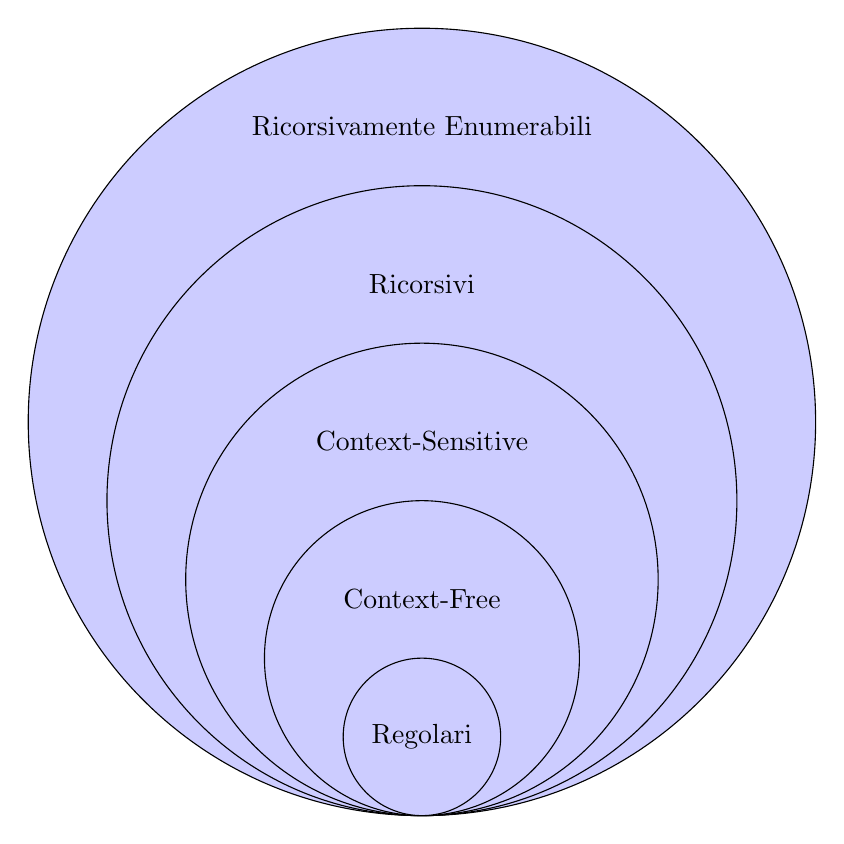
\begin{tikzpicture}[font=\normalsize]
    \coordinate (o) at (0,0);

    \draw (o) -- ++(0,4cm) [fill=blue!20]
    circle (5cm)
    node [align=center, anchor=north, yshift=4cm]{Ricorsivamente Enumerabili};

    \draw (o) -- ++(0,3cm) [fill=blue!20]
    circle (4cm)
    node [align=center, anchor=north, yshift=3cm, dotted]{Ricorsivi};

    \draw (o) -- ++(0,2cm) [fill=blue!20]
    circle (3cm)
    node [align=center, anchor=north, yshift=2cm]{Context-Sensitive};

    \draw (o) -- ++(0,1cm) [fill=blue!20]
    circle (2cm)
    node [align=center, anchor=north, yshift=1cm]{Context-Free};

    \draw (0,0) [fill=blue!20]
    circle  (1cm)
    node {Regolari};

  \end{tikzpicture}
\end{center}

\begin{tblr}{
  hlines, vlines,
  rows ={6mm}, columns = {60mm,c},
  row{1}={primary!80!white}
  % colspec={X[c]X[c]X[c]}
}
  \SetCell[c=1]{c} Linguaggi & \SetCell[c=1]{c} Grammatiche & \SetCell[c=1]{c} Automi \\

  \SetCell[c=1]{c} Regolari & \SetCell[c=1]{c} Regolari
  \begin{itemize}
    \item \(X \to aY, \quad X,Y \in V\);
    \item \(X \to a, \;\;\quad a \in \Sigma\);
    \item \(X \to \varepsilon\);
  \end{itemize} & \SetCell[c=1]{c} DFA \\

  \SetCell[c=1]{c} Context-Free & \SetCell[c=1]{c} Context-Free
  \begin{itemize}
    \item \(X \to w, \quad X \in V, w \in \rbrakets{V \cup \Sigma}^*\)
  \end{itemize} & \SetCell[c=1]{c} PDA \\

  \SetCell[c=1]{c} Context-Sensitive & \SetCell[c=1]{c} Context-Sensitive
  \begin{itemize}
    \item \(\alpha X\beta \to \alpha w \beta, \quad X \in V, \alpha, w, \beta \in \rbrakets{V \cup \Sigma}^*, w \neq \varepsilon\)
  \end{itemize} & \SetCell[c=1]{c} Macchine di Turing limitate linearmente \\

  \SetCell[c=1]{c} Ricorsivi & \textit{Non nota} & \SetCell[c=1]{c} Macchine di Turing terminanti \\

  \SetCell[c=1]{c} Ricorsivamente Enumerabili & \SetCell[c=1]{c} Senza restrizioni
  \begin{itemize}
    \item \(u \to w, \quad u,w \in \rbrakets{V \cup \Sigma}^*\)
  \end{itemize} & \SetCell[c=1]{c} Macchine di Turing \\
\end{tblr}
